\documentclass{article}[12pt;letterpaper]
\usepackage{graphicx}
\usepackage{verbatim}
\usepackage{color}
\usepackage[nohead,nofoot,left=1in,right=1in,top=1in,bottom=1in]{geometry}

\pagestyle{empty}
\raggedright
\frenchspacing
\setlength{\parskip}{0in}
\setlength{\parindent}{0in}

\begin{document}

\begin{flushleft}
Parry Wilcox \\
Andrew Shen
\end{flushleft}

\section{Thread count scaling}

We ran \texttt{nbody -s 1352723313 -nt \$NTHREADS} for \texttt{\$NTHREADS = 1,
2, 4, 8}. For the most part we see the speedup that we expect from using more
threads:

\begin{tabular}{c l}
Thread Count & Time (s) \\
\hline{}
1 & 4.138442 \\
2 & 1.048486 \\
4 & 0.539792 \\
\end{tabular}

For eight cores, we saw some unusual behavior. For most runs, we observed a
slight decrease in performance with the correct results:

\begin{tabular}{l l l l l l l l}
0.559210 & 0.553203 & 0.573746 & 0.564950 &
0.581025 & 0.562103 & 0.562194 & 0.545826
\end{tabular}

But for some runs, particularly immediately consecutive runs, we saw that not
only did the performance decrease, but the integrity of the results was also
compromised:

\begin{verbatim}
###### 4 threads 

dt: 0.0005
Simulation box size: 0.715542
Random seed is 1352723313
# particles : 1024
Using static BLOCK decomposition
Nsteps: 1000

n = 1024, nsteps = 1000
(u,vMax) = ( 9.99816007e-01, 9.97788041e-01 )
(u,vL2 ) = ( 5.74424367e-01, 5.76119911e-01 )
Running time = 5.39792000e-01 sec.

###### 8 threads 

dt: 0.0005
Simulation box size: 0.715542
Random seed is 1352723313
# particles : 1024
Using static BLOCK decomposition
Nsteps: 1000

n = 1024, nsteps = 1000
(u,vMax) = ( 3.49390795e+03, 1.23453369e+04 )
(u,vL2 ) = ( 1.09315048e+02, 3.85857235e+02 )
Running time = 5.44501000e-01 sec.
\end{verbatim}

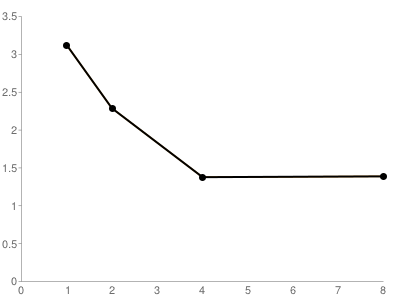
\includegraphics[width=0.3in]{a2_sec1_1.png}

We get a similar result when we use the \texttt{-b} flag for irregular
particle distribution (\texttt{nbody -b -s 1352723313 -nt \$NTHREADS}):

\begin{tabular}{c l}
Thread count & Time (s) \\
\hline{}
1 & 3.120088 \\
2 & \textcolor{red}{segmentation fault} \\ % FIXME!
4 & 0.175171 \\
8 & 0.351271
\end{tabular}

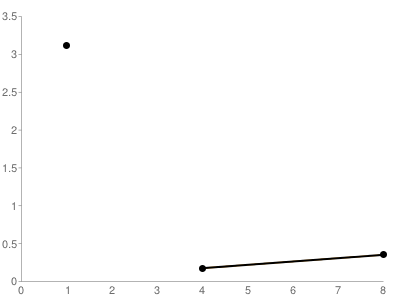
\includegraphics[width=0.3in]{a2_sec1_2.png}

\section{Chunk-scheduled scaling}

\end{document}
